\documentclass[12pt]{article}
\usepackage{latexsym,amssymb,amsmath} % for \Box, \mathbb, split, etc.
% \usepackage[]{showkeys} % shows label names
\usepackage{cite} % sorts citation numbers appropriately
\usepackage{path}
\usepackage{url}
\usepackage{verbatim}
\usepackage[pdftex]{graphicx}
\usepackage{color}

\usepackage{multicol}
\usepackage{fullpage}

% horizontal margins: 1.0 + 6.5 + 1.0 = 8.5
\setlength{\oddsidemargin}{0.0in}
\setlength{\textwidth}{6.5in}
% vertical margins: 1.0 + 9.0 + 1.0 = 11.0
\setlength{\topmargin}{0.0in}
\setlength{\headheight}{12pt}
\setlength{\headsep}{13pt}
\setlength{\textheight}{625pt}
\setlength{\footskip}{24pt}

\renewcommand{\textfraction}{0.10}
\renewcommand{\topfraction}{0.85}
\renewcommand{\bottomfraction}{0.85}
\renewcommand{\floatpagefraction}{0.90}

\makeatletter
\setlength{\arraycolsep}{2\p@} % make spaces around "=" in eqnarray smaller
\makeatother

% change equation, table, figure numbers to be counted inside a section:
\numberwithin{equation}{section}
\numberwithin{table}{section}
\numberwithin{figure}{section}

% begin of personal macros
\newcommand{\half}{{\textstyle \frac{1}{2}}}
\newcommand{\eps}{\varepsilon}
\newcommand{\myth}{\vartheta}
\newcommand{\myphi}{\varphi}

\newcommand{\IN}{\mathbb{N}}
\newcommand{\IZ}{\mathbb{Z}}
\newcommand{\IQ}{\mathbb{Q}}
\newcommand{\IR}{\mathbb{R}}
\newcommand{\IC}{\mathbb{C}}
\newcommand{\Real}[1]{\mathrm{Re}\left({#1}\right)}
\newcommand{\Imag}[1]{\mathrm{Im}\left({#1}\right)}

\newcommand{\norm}[2]{\|{#1}\|_{{}_{#2}}}
\newcommand{\abs}[1]{\left|{#1}\right|}
\newcommand{\ip}[2]{\left\langle {#1}, {#2} \right\rangle}
\newcommand{\der}[2]{\frac{\partial {#1}}{\partial {#2}}}
\newcommand{\dder}[2]{\frac{\partial^2 {#1}}{\partial {#2}^2}}

\newcommand{\nn}{\mathbf{n}}
\newcommand{\xx}{\mathbf{x}}
\newcommand{\uu}{\mathbf{u}}

\newcommand{\junk}[1]{{}}

% set two lengths for the includegraphics commands used to import the plots:
\newlength{\fwtwo} \setlength{\fwtwo}{0.45\textwidth}


\renewcommand{\labelitemi}{}
\renewcommand{\labelitemii}{}
\renewcommand{\labelitemiii}{}


% end of personal macros
% \input{inputFile.tex}


\begin{document}
\DeclareGraphicsExtensions{.jpg}



\begin{center}
\textbf{\Large AAAI Fellowship Application}\\[12pt] 
%\textbf{\Large } \\[6pt]
%\textbf{\Large } \\[6pt]
John Oberlin\\
Brown University, 2014\\
\end{center}

\section{Dissertation Abstract}
%Imagine handing ten everyday objects to your robot assistant, who then proceeds to
%scan them and put them where they belong. Now think of a situation where a capable
%robot might improve someone's life by helping a disabled person prepare a meal,
%fetching a purse or storing a book for a bedridden patient, or handing ointment
%to a busy parent whose hands are full taking care of their child.

Robots have the potential to help people by making changes to the physical world.
A robot assistant could improve someone's life by helping a disabled person prepare a meal,
fetching a purse for a bedridden patient, or handing ointment
to a busy parent whose hands are full taking care of their child. As a matter of course,
if a robot is going to affect the world it must have an understanding of the positions
of objects. Computer vision is an appealing route for obtaining this understanding, as RGB-D
sensors are cheaper and more familiar than most alternatives.

State of the art techniques in object detection and pose estimation
are powerful and general but usually run at a rate much less than 1 Hz and require
time and expertise to build, maintain, and operate. The high demands of modern systems
can make it difficult to employ such techniques in real-time human-robot interaction.
Although effective solutions exist for category recognition, there is no off-the-shelf
framework for object detection, segmentation and pose estimation that allows new objects
to be quickly and easily added by non-experts.

Popular techniques for real-time detection use modified deformable part models (DPMs) \cite{kostas1} \cite{forsyth1},
and sometimes exploit different channels of data \cite{dietr1} \cite{sliding1}.  
These approaches have seen success in their target domains, but are too technical for general
application and need to be integrated with interactive systems. A computer 
vision system that is simple, reliable, and easy to use with ROS (Robot Operating System)
would benefit many researchers.

The aim of my dissertation at Brown is to enable a robot
to autonomously scan 10 novel objects in order to construct robust models for detection,
pose estimation, grasping, and manipulation of those objects during collaborations with
a human operator. We propose the following work-flow for this task: 1.) A human operator provides
the robot with a box of objects. 2.) The robot picks up each object and scans it from many different
perspectives to collect appearance data. 3.) The robot trains classifiers to recognize each object. 
4.) The robot collects labels and meta data for the objects from Amazon Mechanical Turk. 5.) The
robot can detect the objects in the environment and accurately respond to an operator's request
to fetch an object or put it away.

Our prototype system detects and estimates poses of objects in RGB-D video taken with a Kinect and
runs at a frequency of 2 Hz. Our detection framework
% uses a box metaphor to talk about space in a way that is amenable to 
calculates three quantities for each frame $f$ which facilitate
planning and reasoning. 

The first quantity is a subset $\mathcal{G}_f$ of pixel locations, which induces a grid graph whose nodes
correspond to points spaced $s=5$ pixels apart in the input image $f$ and whose edges connect each pixel to its
four cardinal neighbors in the grid. A pixel $g$ is included in $\mathcal{G}_f$ if the local average Objectness (see below)
exceeds a threshold. 
%We manually tune the threshold at the moment, but it would be natural to use a
%max-entropy approach such as herding \cite{herding} to adaptively control it.
The second quantity is $\mathcal{B}_f$, a list of the connected components of the graph induced by $\mathcal{G}_f$.
The third quantity is $\mathcal{R}_f$, a labeling which associates with each point $g \in \mathcal{G}_f$ a token
corresponding to the object instance depicted at that pixel location.

In other words, $\mathcal{G}_f$ denotes areas in the image that probably belong to an object, 
$\mathcal{B}_f$ encodes clusters of pixels which likely correspond to individual objects, and $\mathcal{R}_f$
segments $\mathcal{G}_f$ into object instances, which may involve breaking apart the clusters in $\mathcal{B}_f$.

We determine $\mathcal{G}_f$ using an Objectness measure \cite{bing}, extract features with SIFT \cite{sift} 
and k-means, and perform k-nearest neighbors classification on crops $C_B$ and $C_R$ induced by the
bounding boxes of components in $\mathcal{B}_f$ and $\mathcal{R}_f$.
We currently optimize the objective function for $\mathcal{R}_f$ using a variant of the wide-scale random noise algorithm in \cite{wsrn}.
Our system publishes detections and pose estimates for the crops $C_B$ and $C_R$ on separate topics in ROS. 

To provide accurate help
to a human partner, the robot needs to know how to manipulate objects and understand their typical uses.
Our system will address this issue by inferring object affordances and inducing an OO-MDP \cite{OOMDP} that the robot
can use for robust planning and object manipulation.

We might achieve better performance when determining $\mathcal{R}_f$
by using more sophisticated techniques that incorporate feedback with the robot's OO-MDP planner in 
order to collect additional data such as viewpoints, grasp information, bounding boxes, or descriptive labels.  
Employing a POMDP \cite{POMDP} to explore the space of bounding boxes in an image is a natural approach to investigate.

\begin{figure}
  \begin{center}
    \begin{tabular}{l c}
      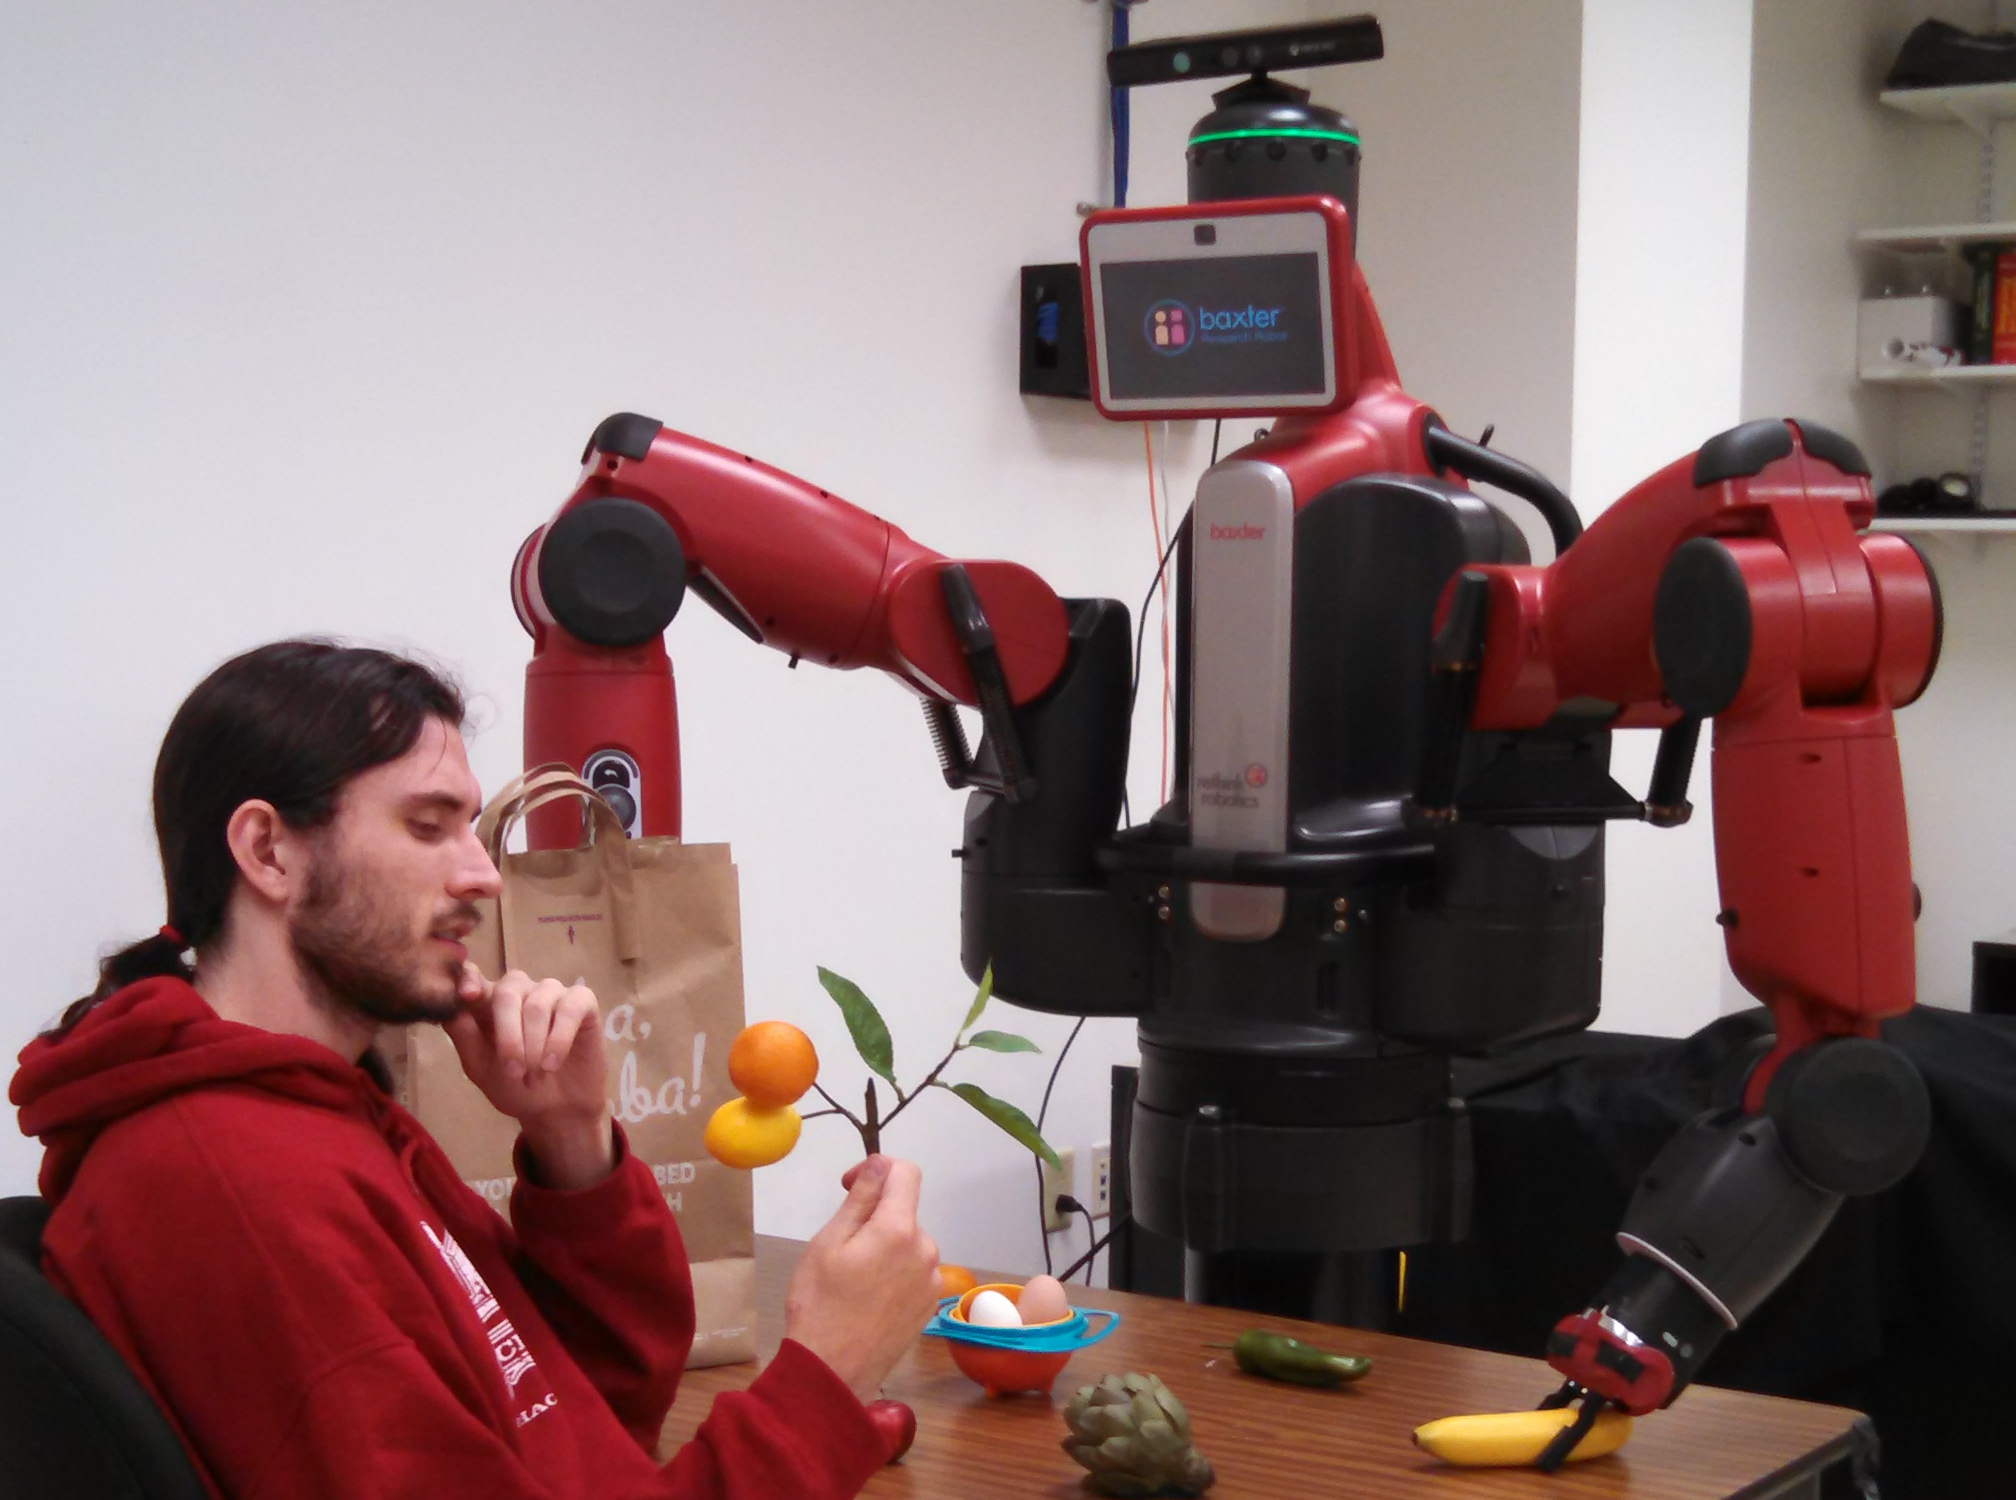
\includegraphics[width=200px, height=150px]{robo2.png} &
      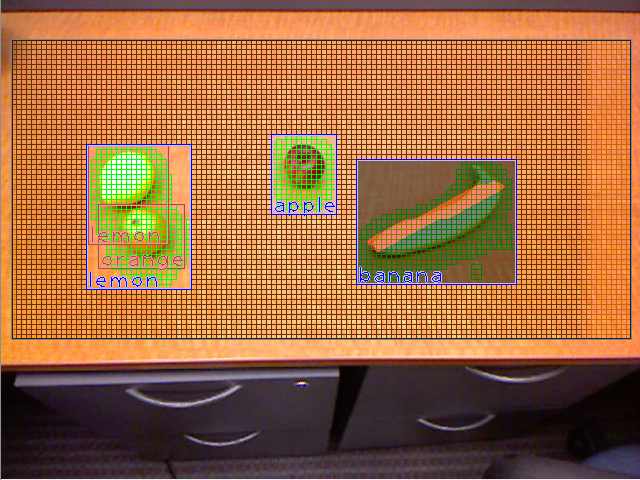
\includegraphics[width=200px, height=150px]{screen2.png} \\
    \end{tabular}
  \end{center}
  \caption{Teaching a robot to identify and manipulate objects can be as easy as bringing home
	    a bag of groceries.}
\end{figure}

%\paragraph{Semi-Automatic Training}
%\begin{enumerate}
  %\item A human operator places the object in a robot's manipulator.
  %\item The operator provides a base pose for the given grasp.
  %\item The robot collects views of many different precisely known poses, together with models for self and background filtering.
%\end{enumerate}

With our prototype system, a computer vision researcher can train accurate models for 5
objects in 15 minutes. Our aim is to integrate a robot into the work-flow so that a novice
user can train 10 objects with 5 minutes of human input.

The framework we have outlined abstracts the detector from the classifier by taking a local notion 
of Objectness and extending it to a global model in a way that allows new detectors 
for local properties to be incorporated seamlessly and without down time.  Our technology 
will enable robots to help humans by robustly sensing and manipulating the objects that people value most.

\newpage

we are bootstrapping proverbially. our philosophy espouses solving weak instances of problems in constrained spaces and using those solutions to create strong solutions in unconstrained spaces.  Thereby, we bootstrap the detection process. To truly be faithful to this approach, we must replace the objectness detector, as it uses an externally trained model. Something like a high sigma DoG or gradient magnitude should do the trick, and it harkens back to Canny.  in fact, we could use a hysteresis step for this as well. this needs to rely on features and algorithms, not data.

We use the language of ensemble learning to speak about obtaining strong solutions to general problems from weak solutions to specific cases of those problems. 

We are not stacking our classifiers in the strictest of senses, but k-means could be considered a subordinate classifier so in that sense we are.  Logistic regression is a likely candidate for a fusion method when classifying windows of states, and so then we might start to truly stack.

We are using bootstrapping to estimate properties such as table orientation and background color. as it turns out, it may be worth investigating bagged nearest neighbors because we approximating it by resampling the data.

We make heavy use of cascades.

Our training method can be viewed as boosting-motivated.

a simpler cascade
sliding window on class
mesh based pose estimator such as ICP

current cascade
objectness
knn-bow class label
knn pose label


proposed 1.0 cascade
objectness
class rapids
knn-bow class candidates
discriminative classifier
pose rapids
knn pose label candidates
discriminative pose estimator

a deep cascade
objectness provides evidence; point cloud and other hooks feed in here
knn-bow class suggestions form blue labels for blue boxes; planning can place contextual clues here by providing suggestions
restricted discriminative classifier (svm or other) forms red label for red boxes; planning can, for instance, fix a red label 
generative model with volumetric representation classifies pose and accounts objectness evidence, depth information and object labels (in the case of parts and compound objects, this includes dynamics information like constraints)
relevant actions are proposed, and activities can then be classified in their own arc. there might be an action happening at these objects.

the notion of rapids (knn -> svm -> fit) can be naturally motivated by the visual system, as has been noted before with BoW and SBoW (http://www.cs.unc.edu/~lazebnik/publications/pyramid_chapter.pdf).

affordances facilitate cascade arrangement. make sure to talk about viola-jones.

an appealing approach is to train the SVM only on the examples proposed by the kNN models.

time is segmented into phrases with relative frames (such as boundary frames) saved as observations. most observations are incomplete, but we can tell which examples we can use for which training tasks.  it is an affordance.

there are certain facets of the world which afford actions that are useful to us during training. the table and the pointer afford labeling the objects with orientations. tables and grounds afford orienting yourself with the world. you could drop an object to find “down”. the image background affords object segmentation.

our teaching framework incorporates signs with affordances to streamline the process of data collection.

each degree of cascade is appropriate for particular regimes. you can switch regimes in real time to accommodate changing environment complexity or resource availability.

at each application, planning includes operator input / real time parameter locking.

a detector cache hierarchy emerges with policies. this immediately induces a dual data hierarchy.

system resources can be bounded by the number of red boxes, which conveniently bounds the number of pose detectors (PDs) necessary to keep around at one time. this is a fixed length PD cache. but if PDs act to break a tie, than PD-cache inherits structure from CD-cache

class detectors can be regenerated based on context. there is a CD-cache from red boxes, a CD-cache from context, and a CD-cache from “hard negative” classes.

we teach the system by finding its weaknesses and training it to overcome these weaknesses. we provide a framework for structuring that training in an affordable, scalable way.  we structure the training, the training structures the models.

“I see you’re having trouble picking up gyroBowls. Let’s think about it differently (initialize generic pose model) and practice gazing a bit (train the pose model).”

need to switch to a threadpool model which can then swap resources such as CPUs and GPUs as they become available.

objectness, gradients, and laplacians. consider running objectness on a contrast normalized image. then, consider using gradient and laplacian information as fine grain evidence for the pose rapid. this approach might allow for a principled solution to occlusion.

don’t forget that k-means here is actually a classifier and so we are technically stacking. introducing the background shunt will make that cascade-like. a shunt is a special kind of cascade step which produces something like a mask.

break the observed space into a block representation, possibly with octree encoding weighted according to scale, and use kNN or hashing to search the space for a similar landscape. then use the navigation schemes learned for the closest neighbors. 

then we can begin volumetric modeling of objects. each block has an rgb-a value associated with it, alpha representing the frequency with which depth is observed at that point.
we can apply markov methods to regularize these models. then it would be fast to move to modeling the faces of the blocks with independent filters, treating the faces as patches, to capture texture.

one approach to teaching the robot to move is to teach it a form for each task. each movement in the form should have parameters corresponding to target points, known obstacles, etc.  It should be similar to dealing with character animations in video games. 




\newpage

\bibliographystyle{siam}
\bibliography{proposal}


\end{document}

% TODO 

% cached training

% train posemodels for some objects
  % hershey cocoa

% try Color BoW
